\documentclass[11pt, a4paper]{article}
\usepackage{fullpage}
\usepackage[USenglish]{babel}
\usepackage{graphicx} 
\usepackage[small,bf,hang]{caption2}
\usepackage{hyperref}
\hypersetup{
    colorlinks,
    citecolor=black,
    filecolor=black,
    linkcolor=black,
    urlcolor=black
}

\title{Master Thesis -  Security Aspects in Virtual Networks\\ \textbf{SITREP 10}}
\author{\textbf{Laurent De Wilde} \\ Master of Science in the Applied Computer Science \\ Vrije Universiteit Brussel}
\date{March 16, 2015}

\begin{document}
\maketitle

\section*{Work done}

This is an overview of the work performed in the past week:
\begin{itemize}
\item Theoretical study is finished.
\item Made an appointment with Prof to discuss the practical testing.
\item Transported the pizzaserver from the VUB datacenter to my home by car.
\item Integrated the server into the existing infrastructure.
\item I installed the Hyper-V role on WS2012 R2, using two NIC's: one for the virtual switch and one for monitoring / remote desktop connection. Obviously, I make use of the so-called ``external network'' of Hyper-V. 

The reason I installed Hyper-V (besides XEN) is that, in contrast to XEN, I do not have much experience with Hyper-V and I would like to gain more experiece with it.
\end{itemize}
The figure below visualizes my current network setup.
\begin{figure}[h]
    \centering
    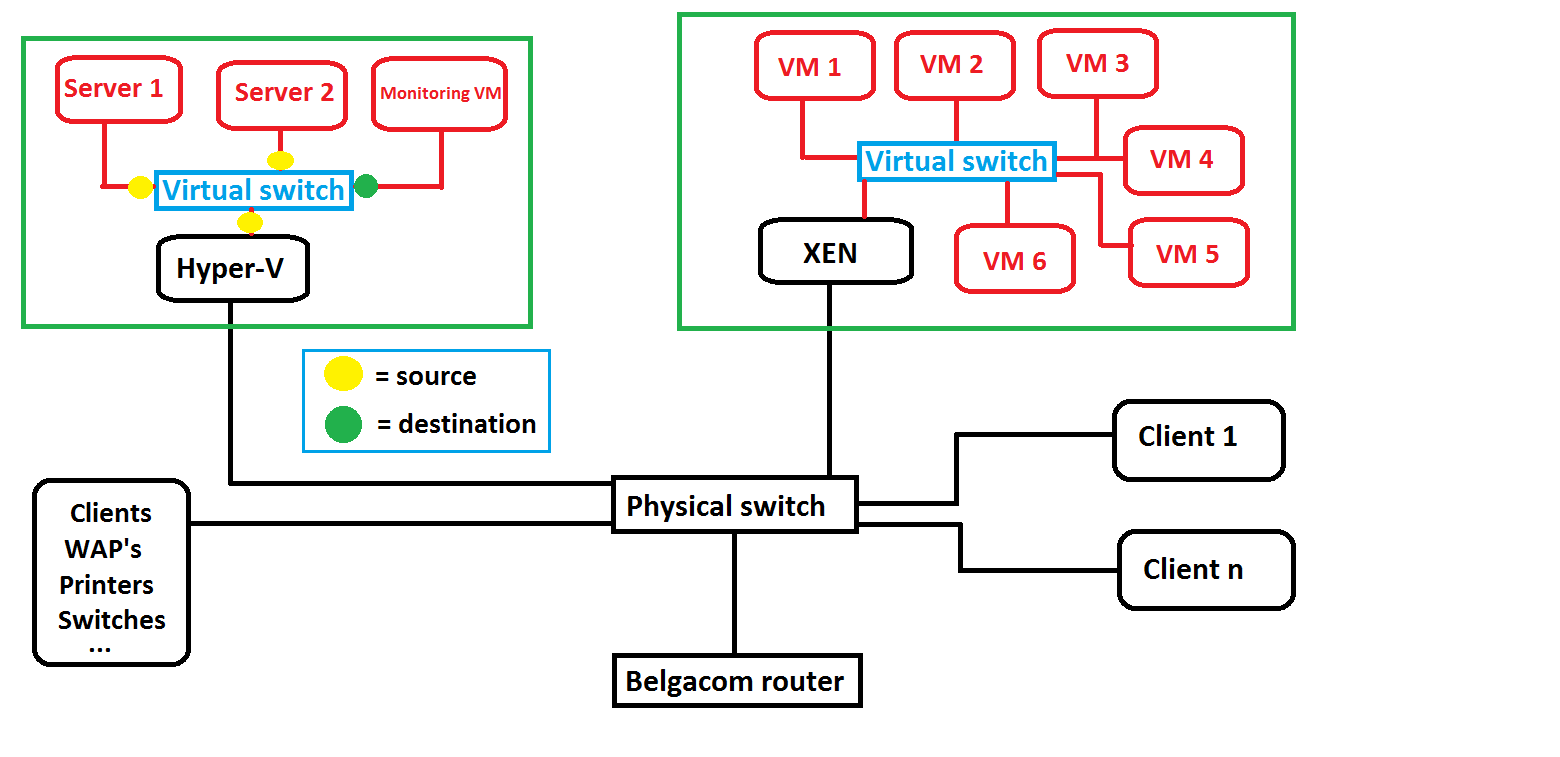
\includegraphics[width=1.05\textwidth]{Network.png}
\end{figure}

\clearpage

\begin{itemize}
\item After the hardware setup was completed, I started configuring Hyper-V: I have setup three VM's and each VM has its own vNIC and is connected to the virtual switch. One of those VM's is used to capture all traffic that passes on all the ports of the switch, hence the name ``monitoring VM''.

As the Prof stated he was very pleased with the dynamic memory feature of Hyper-V, all VM's use dynamic memory.

I was asked if a vNIC is able to capture traffic on the network to later reconstruct the protocols. After some research, it turns out one can use port mirroring for this purpose. So I configured the vPorts of Server 1 and Server 2 on the vSwitch to act as a source. Meaning they make a copy of the traffic to and from those ports and send it to the destination. This destination is Monitoring VM.

After that, I tested the setup. I installed Wireshark on the ``Monitoring VM'' and pinged from ``Server 1'' to ``Server 2'' and watched how Wireshark captured all the ICMP Ping requests and replies - not destinated to the ``Monitoring VM''. So, \textbf{yes}, the vNIC on the ``Monitoring VM'' captured traffic between VM's (inter - VM) on the same physical host and thus act as a sniffer.
\end{itemize}

Below are some screenshots. One can observe that broadcast messages not originating from the Hyper-V VM's are captured as well as some traffic from a XEN VM (the primary DNS server of my domain to be precise).

\begin{figure}[h]
    \centering
    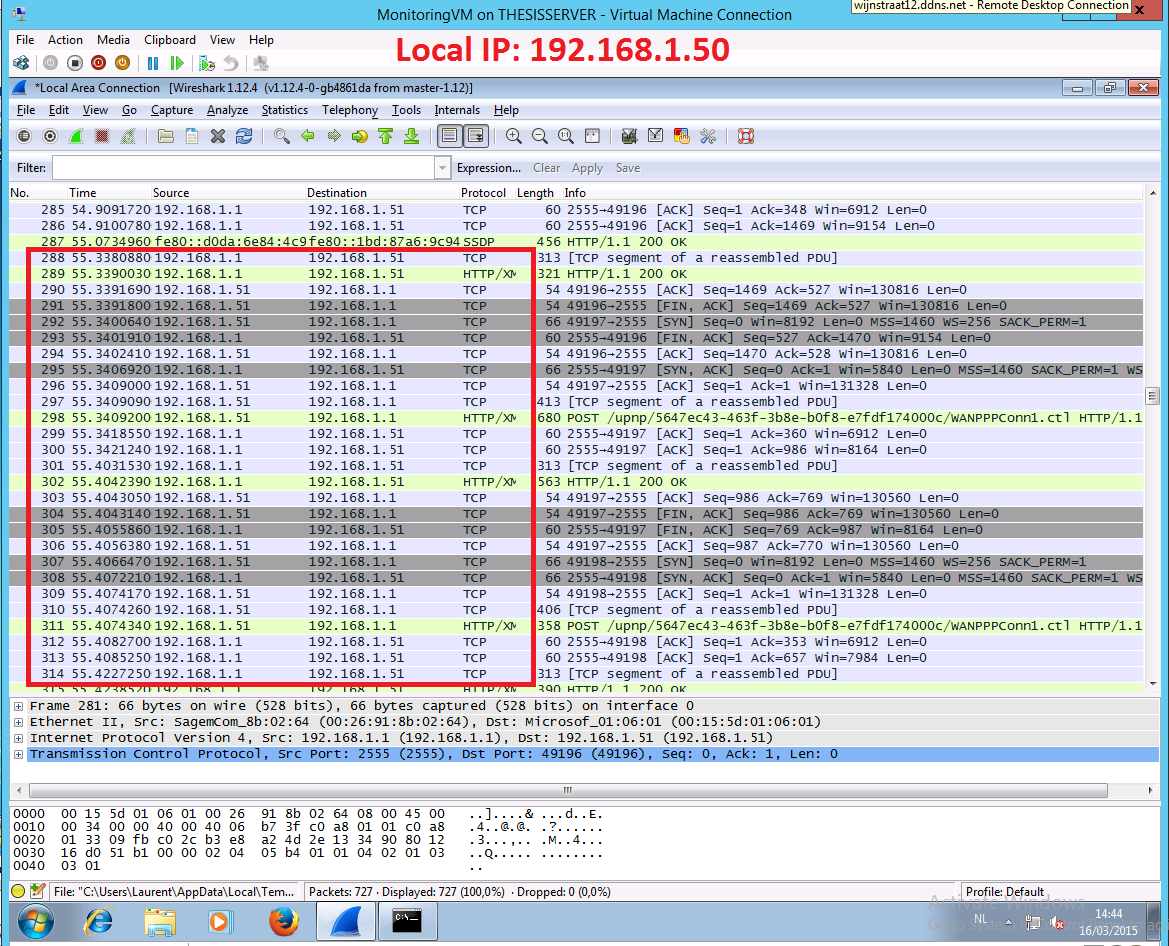
\includegraphics[width=0.9\textwidth]{HyperV_6.png}
   \caption{Traffic between Server 1 (192.168.1.51) and the Belgacom router captured by the vNIC.}
\end{figure}
\clearpage
\begin{figure}[h]
    \centering
    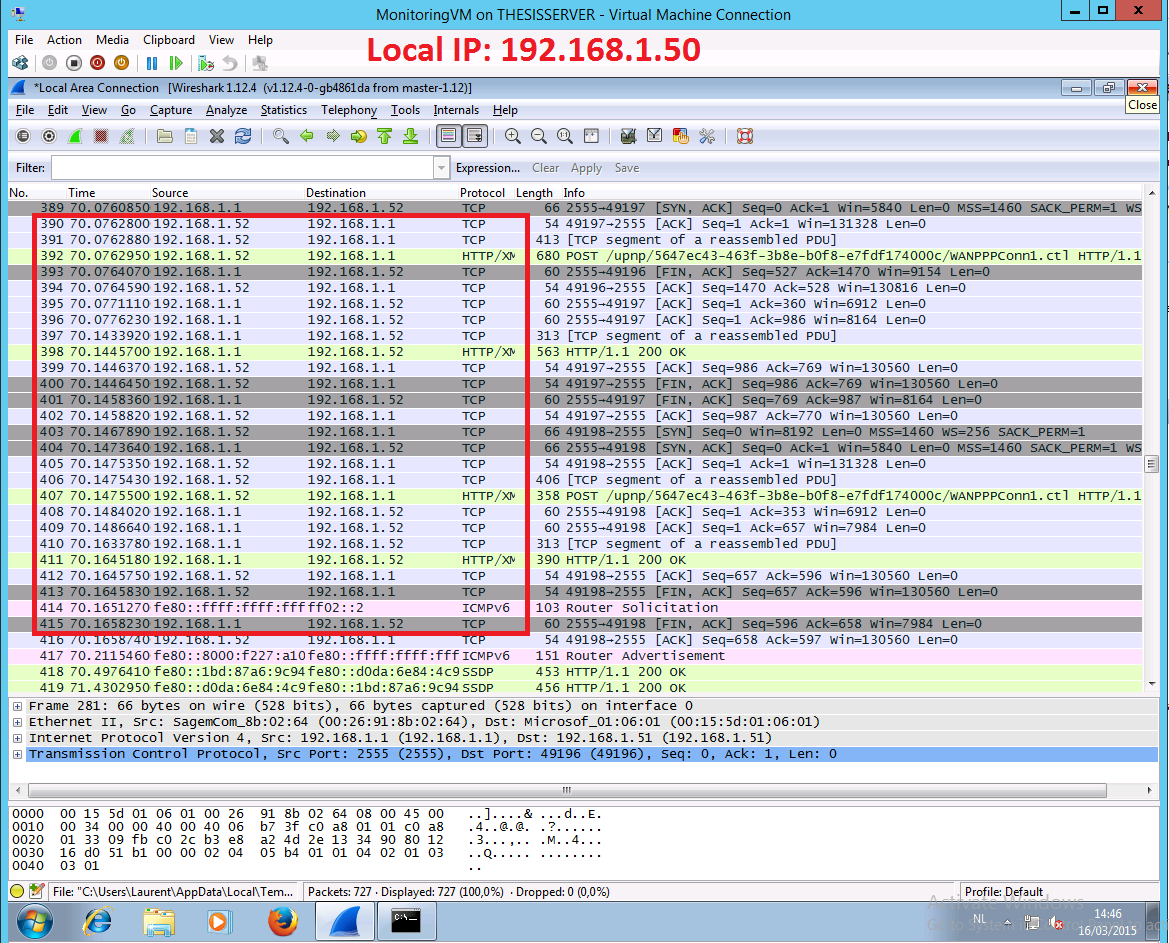
\includegraphics[width=1\textwidth]{HyperV_7.png}
   \caption{Traffic between Server 2 (192.168.1.52) and the Belgacom router captured by the vNIC.}
\end{figure}
\clearpage
\begin{figure}[h]
    \centering
    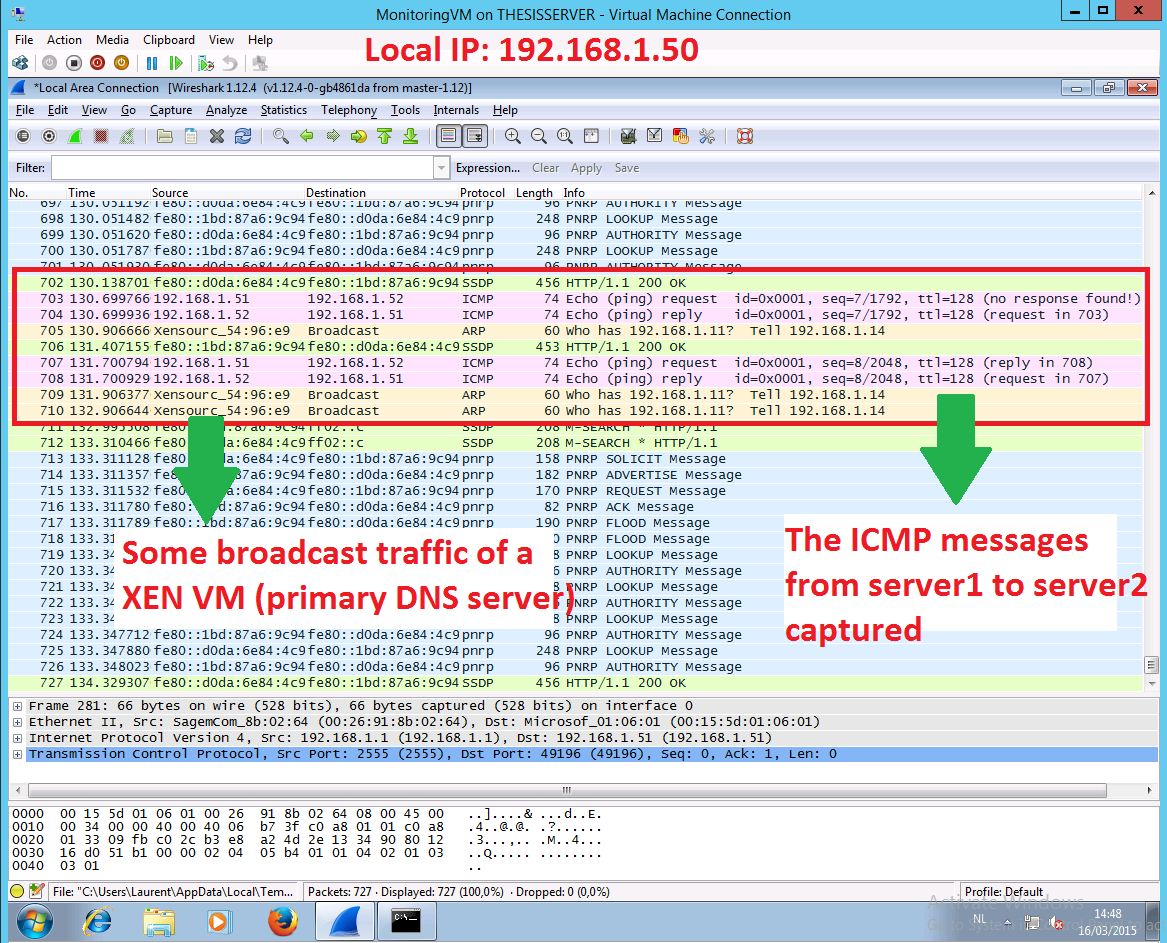
\includegraphics[width=1\textwidth]{HyperV_8.png}
   \caption{ICMP Ping requests captured by the vNIC between server 1 and server 2.}
\end{figure}
\clearpage
\textbf{But what about external traffic to and from external networks to the virtual switch?} \\ \\
So far, I have only tested internal traffic between VM's. I also wanted to test if this ``Monitoring VM" is able to capture traffic orginating from my XEN server or any other client on the network. \\
Therefore, additional settings must be configured on Hyper-V: the physical NIC bound to the vSwitch - that is, the external port of the vSwitch, must be set to ``source'' as well.

This is illustrated in the following figure:
\begin{figure}[h]
    \centering
    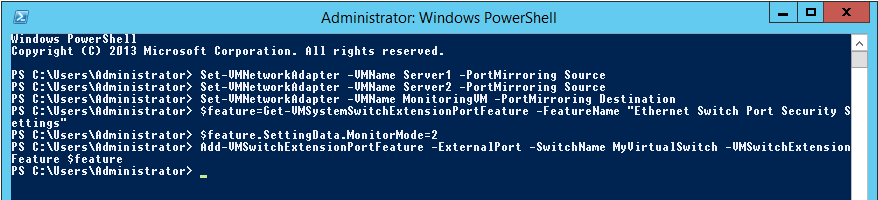
\includegraphics[width=1\textwidth]{HyperV_13.png}
\end{figure}
As it turned out, traffic from a XEN VM to a Hyper-V VM is captured by the ``Monitoring VM''. Also is traffic captured from a XEN VM to the Hyper-V host and traffic is also captured from a Hyper-V VM to the Hyper-V host. Notice that in the screenshots, other IP addresses not originating from the Hyper-V virtual switch appear in the list. This was not the case in the previous samples.
\clearpage
\begin{figure}[h]
    \centering
    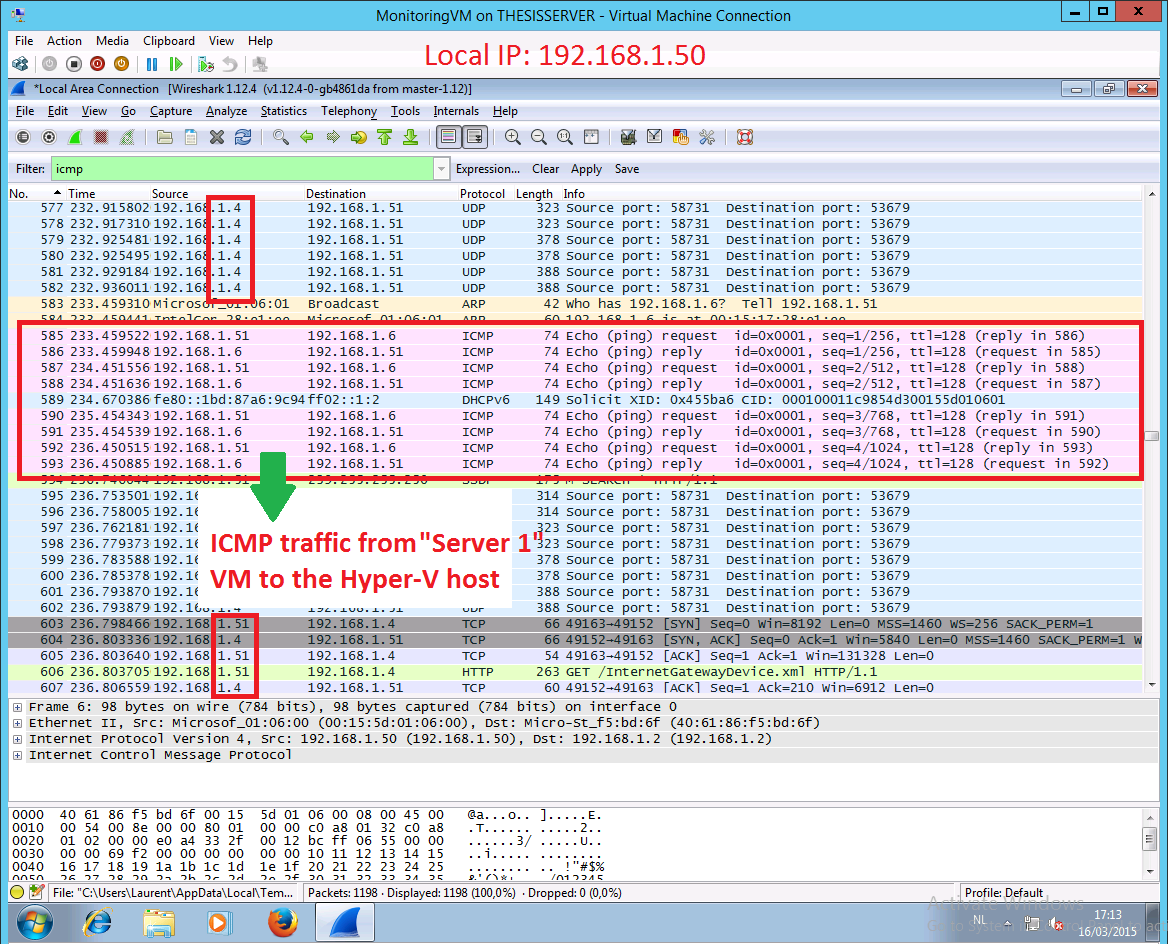
\includegraphics[width=1\textwidth]{HyperV_10.png}
\end{figure}
\clearpage
\begin{figure}[h]
    \centering
    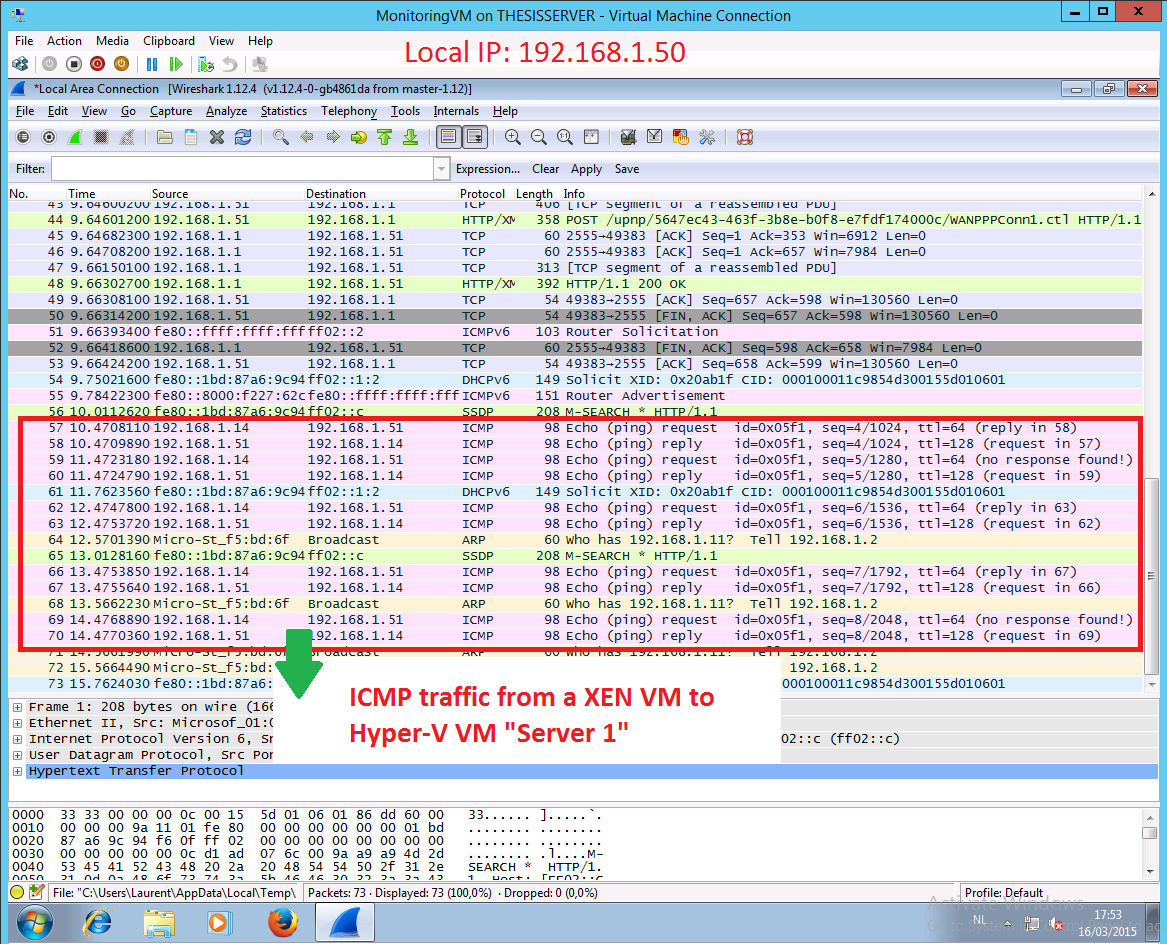
\includegraphics[width=1\textwidth]{HyperV_11.png}
\end{figure}
\clearpage
\begin{figure}[h]
    \centering
    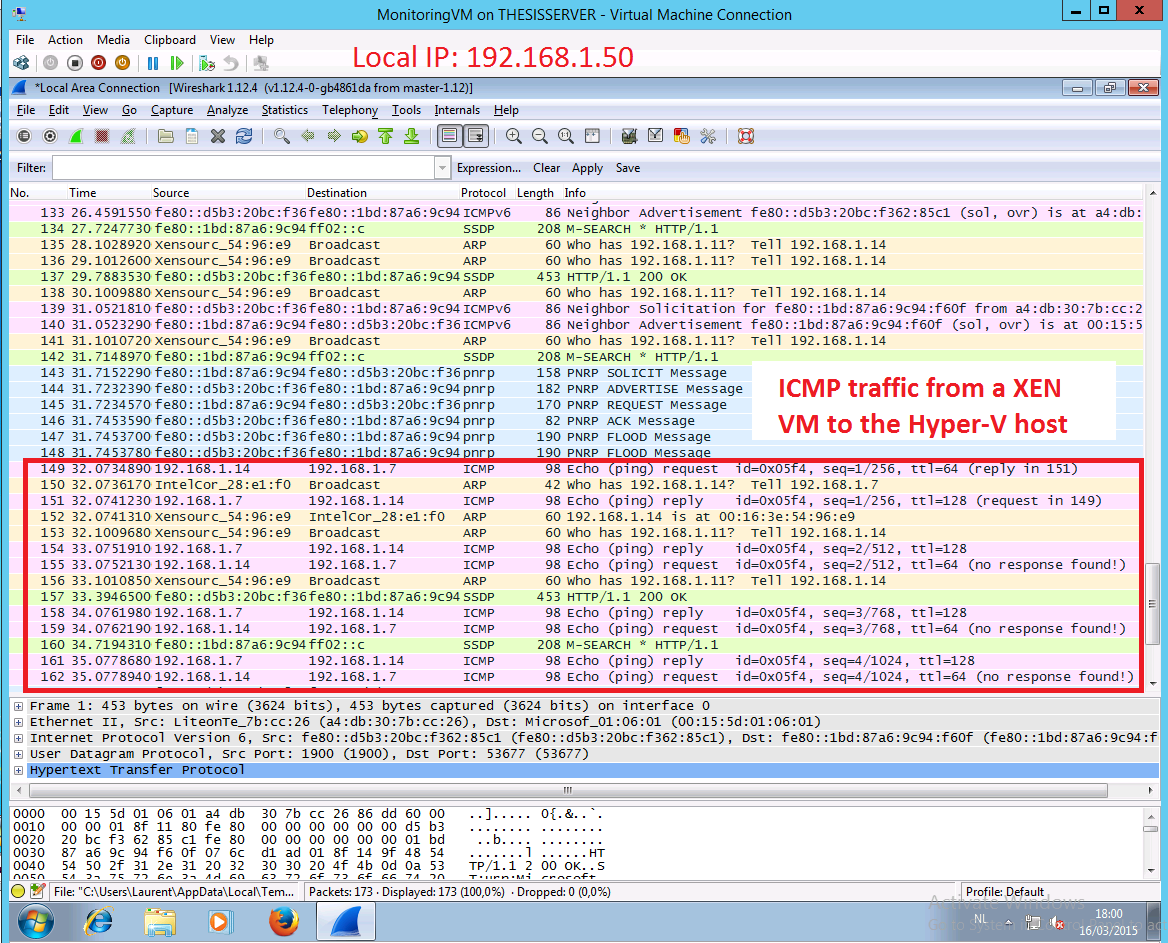
\includegraphics[width=1\textwidth]{HyperV_12.png}
\caption{Traffic from any client to the Hyper-V host is also captured by the VM running on this Hyper-V host.}
\end{figure}
The tests show that it is possible, with some configuration, to snif a virtual switch. It is therefore possible to capture all ports on a vSwitch and forward (make a copy of) the packets to a VM that has a packet sniffer running.

\section*{Planning}
 
This week, or otherwise next week, I plan to install Snort on the virtual network. But before I start with that, I would like to hear the Prof his opinion of the delivered work.


\section*{Problems}



\section*{Issues}

The tests were performed using Hyper-V. If requested, I can do the same with XEN.


\section*{Assistance}

See planning.


\end{document}